\question %9
\emph{Résolvez à nouveau ce modèle en imposant à présent l'intégralité des
variables pour lesquelles c'est absolument indispensable
(utilisez la fonction \texttt{intlinprog}).
Commentez l'allure de la solution obtenue,
et comparez aux solutions obtenues précédemment.}

\begin{figure}[H]
  \begin{center}
    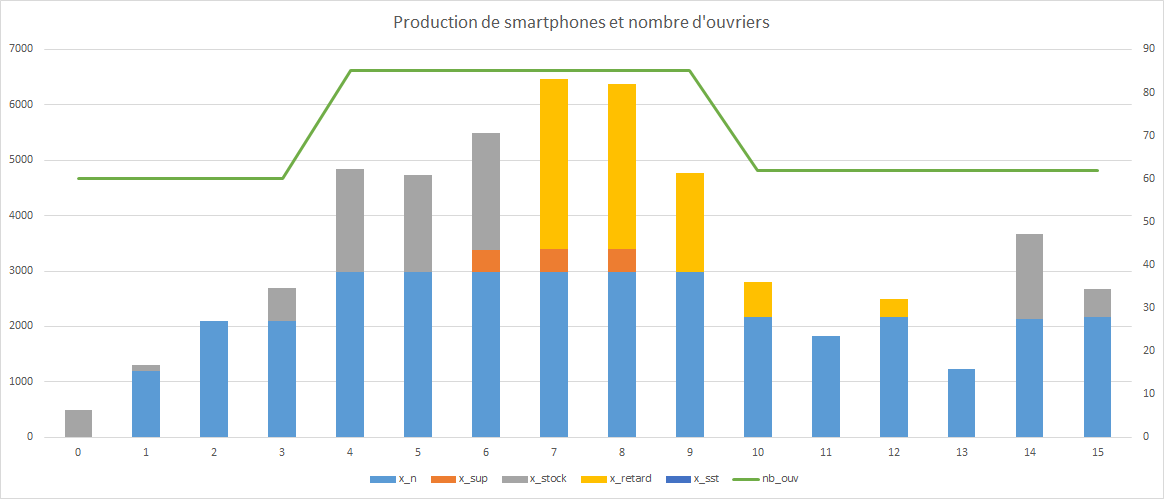
\includegraphics[scale = 0.8]{img/grapheProductionOuv.png}
	  \caption{Répartition du moyen de production des smartphones en fonction des semaines et évolution du nombre d'ouvriers dans le cas entier.}
	  \label{fig:grapheProductionOuv}
  \end{center}
\end{figure}

Les résultats obtenus sont présentés à la figure \ref{fig:grapheProductionOuv}. On observe que la possibilité d'engager et de licencier des ouvriers est bien utilisée. La solution optimale consiste à engager 25 ouvriers pour faire face à l'important pic de demande, puis d'en licencier 23 une fois ce pic dépassé. Cette nouvelle possibilité fait apparaître 3 grande différences entre les solutions : 
\begin{enumerate}
\item Nous ne devons plus faire appel à la sous-traitance.
\item Nous avons beaucoup moins recours aux heures supplémentaires des ouvriers. Ceux-ci n'en effectuent que lors de 3 semaines, comparé à 8 pour le modèle simplifié.
\item Le stock constitué pour faire face au pic de demande est moins important car notre usine peut absorber une plus grande demande.
\end{enumerate}
Il est également intéressant de remarquer que le nombre d'ouvriers ne change que lors de 2 semaines. On n'engage et on ne licencie qu'une seule fois. Ceci est probeblement dû au coût d'embauche et de licenciement et on voit qu'il était donc très important de l'inclure dans le modèle. 

Enfin, le coût a bien baissé grâce à cette nouvelle possibilité. Il est descendu à 3.755.300 unités alors qu'il était de 3.902.000 unités à personnel constant.